% ==========================================================
% 5. 단일 노드 트랜스포머: 순전파와 역전파
% ==========================================================
\section{단일 노드 트랜스포머: 순전파와 역전파}
\label{sec:sn}

이 장에서는 병렬화를 전혀 사용하지 않는 \emph{단일 노드(single-node)} 환경에서
하나의 트랜스포머 레이어가 어떻게 동작하는지 정리한다.
순전파와 역전파 모두에 대해 텐서의 모양과 데이터 흐름을 중심으로 설명하며,
각 구성요소를 분리해서 살펴본다.

다루는 주요 구성 요소는 다음과 같다.
\begin{itemize}
  \item \textbf{입력 임베딩 레이어}: 토큰 ID를 연속 벡터 표현으로 변환.
  \item \textbf{멀티헤드 어텐션(MHA)}: 시퀀스 내 위치들 사이의 어텐션 계산.
  \item \textbf{피드포워드 네트워크(MLP/FFN)}: 위치별 비선형 변환.
  \item \textbf{출력 프로젝션과 손실}: 은닉 상태를 로그릿으로投영하고 손실 계산.
\end{itemize}

우리는 배치 크기가 $B$, 시퀀스 길이가 $S$인 토큰 ID 배치
$\mathbf{T} \in [B,S]$가 주어진다고 가정한다.
레이어 내부의 은닉 표현은 보통
\[
  \mathbf{X} \in \mathbb{R}^{B \times S \times D}
\]
와 같이 표현되며, 여기서 $D$는 모델(은닉) 차원이다.
역전파에서는 스칼라 손실 $\mathcal{L}$에 대한 기울기가
이러한 텐서들과 대응되는 가중치 행렬들을 따라 어떻게 흐르는지를 추적한다.

% ------------------------ 5.0 Overall Layer Flow ---------------------

\subsection{전체 트랜스포머 레이어 흐름}

각 구성 요소를 개별적으로 보기 전에,
단일 노드 트랜스포머 레이어 전체에서 순전파와 역전파가 어떻게 흘러가는지
상위 수준에서 먼저 살펴보자.
Figure~\ref{fig:single_node_overall}은
입력 임베딩으로부터 MHA, MLP, 출력 프로젝션을 거쳐 손실에 이르는
순전파 경로와, 다시 손실에서 역전파되어 입력 임베딩까지 전파되는
기울기 흐름을 한 그림에 요약한 것이다.

\begin{figure}[htbp]
  \centering
  \resizebox{\linewidth}{!}{%
\begin{tikzpicture}[
    node distance=2.5cm,
    >=stealth,
    block/.style={rectangle, draw=black, fill=white, text width=5em, text centered, rounded corners, minimum height=8em, font=\bfseries},
    forward/.style={-{Stealth[length=2mm]}, thick, black},
    backward/.style={-{Stealth[length=2mm]}, thick, black, densely dashed},
    io/.style={text centered, font=\bfseries}
]
    % Title
    \node[font=\Large\bfseries] at (10, 6) {Transformer Overall Flow};

    % Forward path nodes (horizontal)
    \node (input) [io] {$\mathbf{X}$};
    \node (encoding) [block, right of=input, yshift=-3em] {Input\\Encoding};
    \node (mha) [block, right of=encoding] {MHA};
    \node (mlp) [block, right of=mha] {FFN};
    \node (output) [block, right of=mlp] {Output\\Projection};
    \node (pred) [io, right of=output, yshift=3em] {$\mathbf{Y}$};
    \node (loss) [align=center, io, right of=output] {\small LOSS:\\$\mathcal{L}(\mathbf{Y,Y_\text{targets}})$};
    \node (gradient) [io, right of=output, yshift=-3em] {$\mathbf{dY}(=\frac{dL}{dY})$};

    % Forward arrows (upper part of blocks)
    \draw [forward] (input) -- ([yshift=3em]encoding.west);
    \draw [forward] ([yshift=3em]encoding.east) -- ([yshift=3em]mha.west);
    \draw [forward] ([yshift=3em]mha.east) -- ([yshift=3em]mlp.west);
    \draw [forward] ([yshift=3em]mlp.east) -- ([yshift=3em]output.west);
    \draw [forward] ([yshift=3em]output.east) -- (pred);
    \draw [forward] (pred) -- (loss);
    \draw [backward] (loss) -- (gradient);

    % Backward arrows (lower part of blocks)
    \draw [backward] (gradient) -- ([yshift=-3em]output.east);
    \draw [backward] ([yshift=-3em]output.west) -- ([yshift=-3em]mlp.east);
    \draw [backward] ([yshift=-3em]mlp.west) -- ([yshift=-3em]mha.east);
    \draw [backward] ([yshift=-3em]mha.west) -- ([yshift=-3em]encoding.east);

    % Brace for layer repetition
    \draw[decorate, decoration={brace, amplitude=10pt}]
        ([yshift=3.5em]mha.north west) -- ([yshift=3.5em]mlp.north east)
        node[midway, above=12pt, font=\normalsize] {$N$ layers};

    % Labels (Legend)
    \coordinate (legend) at ([xshift=-1.5cm, yshift=6.5em]input);
    \draw[forward] (legend) -- ++(0.8,0) node[right, font=\normalsize] {Forward};
    \draw[backward] ([yshift=-0.6cm]legend) -- ++(0.8,0) node[right, font=\normalsize] {Backward};

\end{tikzpicture}%
}
  \caption{단일 노드 트랜스포머 레이어의 전체 순전파 및 역전파 흐름.
  실선 화살표는 순전파 활성값을, 점선 화살표는 손실 $\mathcal{L}$로부터
  출력 프로젝션, MLP, MHA를 거쳐 입력 임베딩으로 되돌아가는 기울기 흐름을
  나타낸다.}
  \label{fig:single_node_overall}
\end{figure}


% ------------------------ 5.1 Input Embedding ------------------------

\subsection{입력 임베딩 레이어}

입력 임베딩 레이어는 이산적인 토큰 ID를 연속 벡터 표현으로 변환하여,
트랜스포머 스택의 첫 번째 은닉 상태
$\mathbf{X} \in \mathbb{R}^{B \times S \times D}$를 만들어낸다.
다음과 같은 파라미터를 사용한다고 가정한다.
\begin{itemize}
  \item 토큰 임베딩 행렬 $\mathbf{E} \in \mathbb{R}^{V \times D}$:
        $V$는 어휘(vocabulary) 크기.
  \item 위치 임베딩 테이블 $\mathbf{P} \in \mathbb{R}^{S \times D}$:
        학습 가능한 테이블이거나 사인/코사인 기반의 고정 테이블.
\end{itemize}

토큰 ID 배치 $\mathbf{T} \in [B,S]$가 주어졌을 때, 임베딩 레이어는 개념적으로
다음과 같은 연산을 수행한다.
\begin{itemize}
  \item 각 위치 $(b,s)$에 대해 토큰 ID $\mathbf{T}[b,s]$를
        토큰 임베딩 행렬 $\mathbf{E}$의 해당 행으로 매핑하여
        토큰 임베딩 벡터를 얻는다.
  \item 시퀀스 위치 $s$에 대응하는 위치 임베딩 $\mathbf{P}[s,:]$를
        토큰 임베딩에 더한다.
  \item 필요하다면 드롭아웃을 적용하여 초기 은닉 상태
        $\mathbf{X} \in [B,S,D]$를 얻는다.
\end{itemize}

\begin{figure}[htbp]
  \centering
  \documentclass{article}

\usepackage{amsmath, amssymb}
\usepackage{tikz}
\usepackage{graphicx}
\usepackage{caption}
\usepackage[margin=1in, landscape]{geometry}
\usetikzlibrary{shapes, arrows, positioning, fit, calc}

\begin{document}

% ---------- Input Embedding -> (to MHA) ----------
\noindent
\resizebox{\linewidth}{!}{%
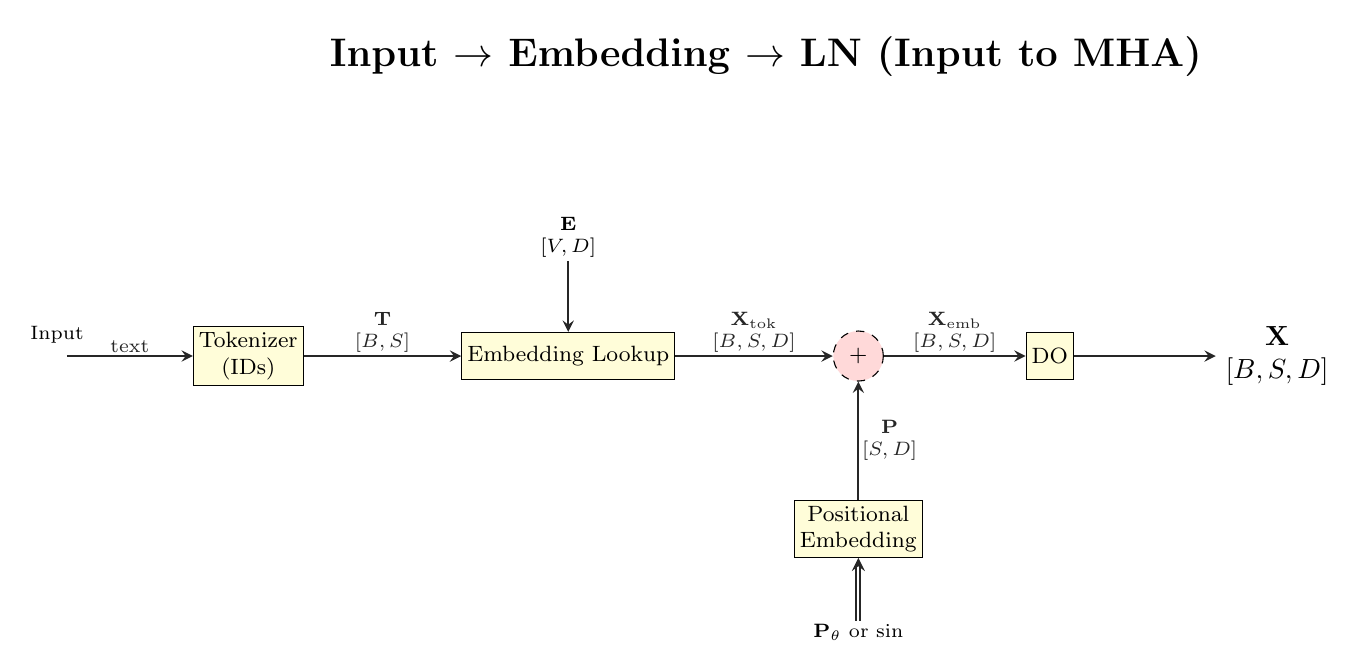
\begin{tikzpicture}[
  >=stealth,
  auxnode/.style={draw, rectangle, fill=yellow!15, minimum height=6mm, inner sep=2pt, font=\footnotesize, align=center},
  mulnode/.style={draw, circle, fill=green!15, minimum size=6mm, font=\footnotesize, align=center},
  addnode/.style={draw, circle, dashed, fill=red!15, minimum size=6mm, font=\footnotesize, align=center},
  flow/.style={->, thick, black!85},
  flow2/.style={->, double, thick, black!85},
  dimlabel/.style={font=\scriptsize, inner sep=1pt, align=center}
]

\node[font=\Large\bfseries] at (9, 3.8) {Input $\rightarrow$ Embedding $\rightarrow$ LN (Input to MHA)};

% nodes
\node (RawText) at (0,0) {};
\node[auxnode, align=center] (Tok)   [right=1.6cm of RawText] {Tokenizer\\(IDs)};
\node[auxnode, align=center] (Lookup)[right=2.0cm of Tok]     {Embedding Lookup};
\node[addnode, minimum size=6mm] (Sum) [right=2.0cm of Lookup] {+};
\node[auxnode, align=center] (PosE)  [below=1.5cm of Sum]  {Positional\\Embedding};
\node[auxnode] (Drop) [right=1.8cm of Sum] {DO};
\node (OUTPUT)   [align=center, right=1.8cm of Drop]   {$\mathbf{X}$\\$[B,S,D]$};

% parameter/const “double” edges
\node[dimlabel] (Eparam) [align=center, above=0.9cm of Lookup] {$\mathbf{E}$\\$[V,D]$};
\node[dimlabel] (Pparam) [align=center, below=0.8cm of PosE]   {$\mathbf{P}_{\theta}$ or sin};

% flows
\draw[flow] (RawText) -- (Tok) node[dimlabel, midway, above]
  {$\text{text}$};
\draw[flow] (Tok) -- (Lookup) node[dimlabel, midway, above]
  {$\mathbf{T}$\\$[B,S]$};

% Embedding matrix E
\draw[flow] (Eparam) -- (Lookup);

% Lookup -> Sum (token embeddings)
\draw[flow] (Lookup) -- (Sum) node[dimlabel, midway, above]
  {$\mathbf{X}_{\text{tok}}$\\$[B,S,D]$};

% Positional embedding path
\draw[flow] (PosE) -- (Sum) node[dimlabel, midway, right]
  {$\mathbf{P}$\\$[S,D]$};

% Optional: show P as parameter (sinusoidal/learned)
\draw[flow2] (Pparam) -- (PosE) ;

\draw[flow] (Sum) -- (Drop) node[dimlabel, midway, above]
  {$\mathbf{X}_{\text{emb}}$\\$[B,S,D]$};
\draw[flow] (Drop) -- (OUTPUT);

% labels for start and destination
\node[dimlabel, above=0.0cm of RawText] {Input};

\end{tikzpicture}%
}

\newpage
\renewcommand{\arraystretch}{1.2}
\small

% -------- Operations (Ops) --------
\begin{center}
\textbf{Operations (Ops)}
\begin{tabular}{llll}
\hline
\textbf{Abbrev} & \textbf{Name} & \textbf{Type / Shape} & \textbf{Notes} \\
\hline
Tokenizer & Tokenizer (IDs) & op & Maps raw text $\to$ integer ids $\mathbf{T}\in\mathbb{Z}^{[B,S]}$. \\
Embedding Lookup & Embedding Lookup & op & Gathers rows from $\mathbf{E}\in\mathbb{R}^{V\times D}$ using ids $\mathbf{T}$. \\
$+$ & Element-wise Add (dashed circle) & op & Adds token and positional embeddings; broadcasting over $B,S$ if needed. \\
DO & Dropout & op & Training-time stochastic dropout on $\mathbf{X}_{\text{emb}}$; identity at inference. \\
\textit{(none)} & Broadcast $\mathrm{BC}_{B,S}(\cdot)$ & op & Expands $[S,D]$ (or $[D]$) to $[B,S,D]$ across batch/sequence. \\
\hline
\end{tabular}
\end{center}

\vspace{0.8em}

% -------- Data Tensors (Values) --------
\begin{center}
\textbf{Data Tensors (Values)}
\begin{tabular}{llll}
\hline
\textbf{Symbol} & \textbf{Name} & \textbf{Shape} & \textbf{Notes} \\
\hline
text & Raw input text & — & Character/byte stream before tokenization. \\
$\mathbf{T}$ & Token ids & $[B,S]$ & Output of Tokenizer; integers in $\{0,\dots,V{-}1\}$. \\
$\mathbf{E}$ & Embedding matrix (params) & $[V,D]$ & Trainable; each vocab entry has a $D$-dim vector. \\
$\mathbf{X}_{\text{tok}}$ & Token embeddings & $[B,S,D]$ & $\mathrm{lookup}(\mathbf{E}, \mathbf{T})$. \\
$\mathbf{P}$ & Positional embedding & $[S,D]$ (or $[B,S,D]$) & Learned $\mathbf{P}_\theta$ \textbf{or} sinusoidal (fixed); broadcast to $[B,S,D]$. \\
$\mathbf{X}_{\text{emb}}$ & Sum of token+pos & $[B,S,D]$ & $\mathbf{X}_{\text{tok}} + \mathrm{BC}_{B,S}(\mathbf{P})$. \\
$\mathbf{X}$ & Input to MHA & $[B,S,D]$ & After dropout (DO); goes to LN/MHA stack. \\
$\mathbf{P}_\theta$ & Learned pos. params & matches $\mathbf{P}$ & Used when positions are trainable; otherwise “sin” denotes fixed sinusoidal. \\
\hline
\multicolumn{4}{l}{\textbf{Shape symbols:}\; $B$=batch size,\; $S$=sequence length,\; $D$=model dim,\; $V$=vocab size.} \\
\multicolumn{4}{l}{\textbf{Notes:}\; In practice, $\mathbf{P}$ may be pre-broadcast to $[B,S,D]$ or added per-token with implicit broadcasting.} \\
\hline
\end{tabular}
\end{center}

\end{document}

  \caption{입력 임베딩 레이어의 순전파.
  토큰 ID는 임베딩 행렬 $\mathbf{E}$를 통해 토큰 임베딩으로 변환되고,
  위치 임베딩 $\mathbf{P}$가 더해진 뒤, (선택적인) 드롭아웃을 거쳐
  초기 은닉 상태 $\mathbf{X} \in [B,S,D]$를 생성한다.}
  \label{fig:single_node_input_embedding}
\end{figure}

역전파에서는 손실 $\mathcal{L}$에 대한 기울기가
$\mathrm{d}\mathbf{X}$로부터 각 임베딩 파라미터로 전파된다.
토큰 임베딩 행렬 $\mathbf{E}$와 위치 임베딩 테이블 $\mathbf{P}$에 대한 기울기는,
각 위치에서 해당 임베딩이 사용된 횟수를 따라 합산(summing)하여 누적된다.
즉, 같은 토큰 ID나 위치가 여러 번 등장하면,
그 위치들로부터의 기울기가 같은 임베딩 파라미터에 더해진다.

% ------------------------ 5.2 Multi-Head Attention -------------------

\subsection{멀티헤드 어텐션 (MHA)}

멀티헤드 어텐션은 모델이 서로 다른 표현 하위공간에서
여러 위치의 정보를 동시에 참조할 수 있게 해주는 메커니즘이다.
구성 요소 관점에서 보면 다음과 같이 나눌 수 있다.
\begin{itemize}
  \item \textbf{선형 프로젝션}: 입력을 쿼리(Q), 키(K), 값(V)로 투영.
  \item \textbf{스케일된 내적 어텐션}: 쿼리–키 내적을 통해 어텐션 스코어를 계산하고,
        소프트맥스로 정규화한 뒤, 값 벡터의 가중합을 계산.
  \item \textbf{멀티헤드 분할}: $N_H$개의 헤드를 병렬로 처리하며,
        각 헤드의 차원은 $D_h$이고 전체 모델 차원은 $D = N_H D_h$.
  \item \textbf{출력 프로젝션}: 각 헤드 출력을 다시 결합(concatenate)한 뒤,
        모델 차원 $D$로 되돌리는 선형 레이어.
\end{itemize}

\subsubsection{순전파}

MHA 블록의 입력은 이전 블록(입력 임베딩 또는 앞선 레이어)의 출력인
\[
  \mathbf{X} \in \mathbb{R}^{B \times S \times D}
\]
이다.
우리는 다음과 같은 순서를 따른다.

\paragraph{(1) 입력 레이어 정규화.}
먼저 은닉 차원 방향으로 레이어 정규화(layer normalization)를 적용한다.
\[
  \mathbf{X}_{\text{norm}} = \mathrm{LN}(\mathbf{X})
  \in \mathbb{R}^{B \times S \times D}.
\]
레이어 정규화는 학습 가능한 스케일/시프트 파라미터
$\boldsymbol{\gamma}, \boldsymbol{\beta} \in \mathbb{R}^{D}$를 가지지만,
도식에서는 주로 정규화된 활성값 $\mathbf{X}_{\text{norm}}$에 초점을 맞춘다.

\paragraph{(2) Q/K/V 선형 프로젝션.}
정규화된 입력에 세 개의 선형 레이어를 적용하여
쿼리, 키, 값 텐서를 생성한다.
\[
  \mathbf{Q} = \mathbf{X}_{\text{norm}} W_Q, \quad
  \mathbf{K} = \mathbf{X}_{\text{norm}} W_K, \quad
  \mathbf{V} = \mathbf{X}_{\text{norm}} W_V.
\]
각 가중치 행렬은 보통
$W_Q, W_K, W_V \in \mathbb{R}^{D \times D}$ 또는
헤드 차원을 고려한 적절한 모양을 가진다.
이후 표현을 위해
$\mathbf{Q}, \mathbf{K}, \mathbf{V}$를
\[
  \mathbf{Q}, \mathbf{K}, \mathbf{V}
  \in \mathbb{R}^{B \times N_H \times S \times D_h}
\]
와 같이 헤드 차원을 명시적으로 드러내는 형태로 재배열(shaping)한다.

\paragraph{(3) 스케일된 내적 어텐션.}
각 헤드 $h$에 대해, 쿼리와 키의 스케일된 내적을 통해 어텐션 스코어를 계산한다.
\[
  \mathbf{A}[b,h,s,t]
  = \frac{1}{\sqrt{D_h}}\,
    \mathbf{Q}[b,h,s,:] \cdot \mathbf{K}[b,h,t,:],
\]
여기서 $s$는 쿼리 위치, $t$는 키 위치이다.
소프트맥스를 시퀀스 축 $t$에 대해 적용하여
어텐션 가중치 $\mathbf{W}_{\text{att}}$를 얻고,
이를 값 텐서 $\mathbf{V}$에 곱해 각 위치의 출력 벡터를 계산한다.
이 연산들의 결과는
\[
  \mathbf{A}_{\text{heads}}
  \in \mathbb{R}^{B \times N_H \times S \times D_h}
\]
와 같은 형태를 가진다.

\paragraph{(4) 헤드 결합 및 출력 프로젝션.}
헤드 차원 방향으로 모든 헤드를 이어 붙여(concatenate) 하나의 텐서로 만들고,
이를 다시 모델 차원 $D$로 투영하는 선형 레이어를 적용한다.
\[
  \mathbf{A}_{\text{out}} = \mathrm{MHA}(\mathbf{X}) \in \mathbb{R}^{B \times S \times D}.
\]
이 텐서는 이후 MLP 블록으로 전달되는 어텐션 출력이다.
도식에서는 각 엣지에 위에서 설명한 텐서 모양이 함께 표시된다
(Figure~\ref{fig:single_node_mha_forward} 참고).

\begin{landscape}
\begin{figure}[htbp]
  % \centering
  \resizebox{\linewidth}{!}{%
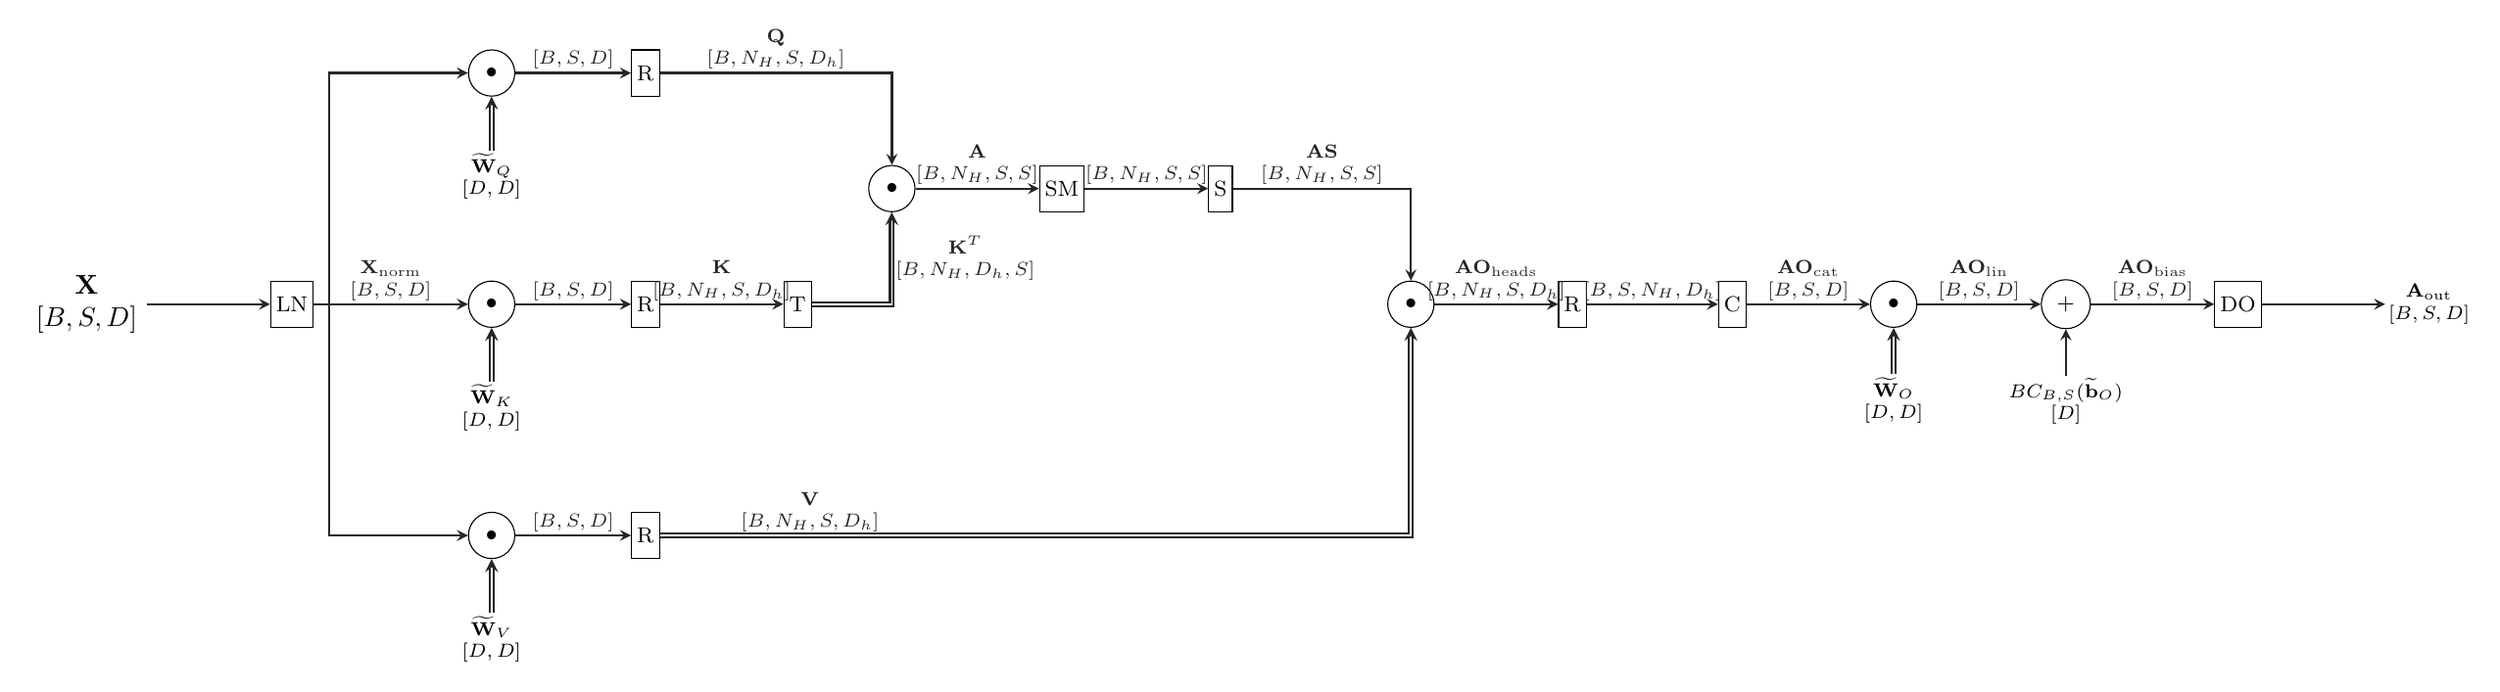
\begin{tikzpicture}[
  every node/.style={transform shape},
  >=stealth,
  auxnode/.style={draw, rectangle, fill=white, minimum height=6mm, inner sep=2pt, font=\footnotesize, align=center},
  mulnode/.style={draw, circle, fill=white, minimum size=6mm, font=\footnotesize, align=center},
  addnode/.style={draw, circle, fill=white, minimum size=6mm, font=\footnotesize, align=center},
  flow/.style={->, thick, black!85},
  flow2/.style={->, double, thick, black!85},
  dimlabel/.style={font=\scriptsize, inner sep=1pt, align=center}
]
% \node[font=\Large\bfseries] at (8, 4.5) {Multi-Head Attention Forward Pass};

\node (Input) at (0.5, 0) [align=center] {$\mathbf{X}$\\$[B,S,D]$};
\node[auxnode] (LN) [right=1.6cm of Input] {LN};

\node[mulnode] (Proj_Q) [right=2.0cm of LN, yshift=3.0cm] {$\bullet$};
\node[auxnode] (R_Q) [right=1.5cm of Proj_Q] {R};

\node[mulnode] (Proj_K) [right=2.0cm of LN, yshift=0cm] {$\bullet$};
\node[auxnode] (R_K) [right=1.5cm of Proj_K] {R};

\node[mulnode] (Proj_V) [right=2.0cm of LN, yshift=-3.0cm] {$\bullet$};
\node[auxnode] (R_V) [right=1.5cm of Proj_V] {R};

\node[dimlabel] (WQ) [align=center, below=0.7cm of Proj_Q] {$\widetilde{\mathbf{W}}_{Q}$\\$[D,D]$};
\node[dimlabel] (WK) [align=center, below=0.7cm of Proj_K] {$\widetilde{\mathbf{W}}_{K}$\\$[D,D]$};
\node[dimlabel] (WV) [align=center, below=0.7cm of Proj_V] {$\widetilde{\mathbf{W}}_{V}$\\$[D,D]$};

\node[auxnode] (T_K) [right=1.6cm of R_K] {T};
\node[mulnode] (QK) [right=2.7cm of R_Q, yshift=-1.5cm] {$\bullet$};
\node[auxnode] (SM) [right=1.6cm of QK] {SM};
\node[auxnode] (Soft) [right=1.6cm of SM] {S};
\node[mulnode] (PV) [right=2.0cm of Soft, yshift=-1.5cm] {$\bullet$};

\node[auxnode] (R_Merge) [right=1.6cm of PV] {R};
\node[auxnode] (Cat) [right=1.7cm of R_Merge] {C};

\node[mulnode] (OProj) [right=1.6cm of Cat] {$\bullet$};
\node[dimlabel] (WO_FWD) [align=center, below=0.6cm of OProj] {$\widetilde{\mathbf{W}}_{O}$\\$[D,D]$};
\node[addnode] (AddB) [right=1.6cm of OProj] {+};
\node[dimlabel] (BO) [align=center, below=0.6cm of AddB] {$BC_{B,S}(\widetilde{\mathbf{b}}_{O})$\\$[D]$};
\node[auxnode] (Drop) [right=1.6cm of AddB] {DO};
\node[dimlabel] (Aout) [align=center, right=1.6cm of Drop] {$\mathbf{A}_{\text{out}}$\\$[B,S,D]$};

\draw[flow] (Input) -- (LN);

\draw[flow] (LN.east) -- ++(0.2,0) |- (Proj_Q.west);
\draw[flow] (LN) -- (Proj_K.west) node[dimlabel, midway, above]{$\mathbf{X}_{\text{norm}}$\\$[B,S,D]$};
\draw[flow] (LN.east) -- ++(0.2,0) |- (Proj_V.west);

\draw[flow2] (WQ) -- (Proj_Q);
\draw[flow2] (WK) -- (Proj_K);
\draw[flow2] (WV) -- (Proj_V);

\draw[flow] (Proj_Q) -- (R_Q) node[dimlabel, midway, above]{$[B,S,D]$};
\draw[flow] (Proj_K) -- (R_K) node[dimlabel, midway, above]{$[B,S,D]$};
\draw[flow] (Proj_V) -- (R_V) node[dimlabel, midway, above]{$[B,S,D]$};

\draw[flow] (R_Q) -| (QK) node[dimlabel, near start, above]{$\mathbf{Q}$\\$[B,N_H,S,D_h]$};
\draw[flow] (R_K) -- (T_K) node[dimlabel, midway, above]{$\mathbf{K}$\\$[B,N_H,S,D_h]$};
\draw[flow2] (T_K) -| (QK) node[dimlabel, near end, right]{$\mathbf{K}^{T}$\\$[B,N_H,D_h,S]$};

\draw[flow] (QK) -- (SM) node[dimlabel, midway, above]{$\mathbf{A}$\\$[B,N_H,S,S]$};
\draw[flow] (SM) -- (Soft) node[dimlabel, midway, above]{$[B,N_H,S,S]$};
\draw[flow] (Soft) -| (PV) node[dimlabel, near start, above]{$\mathbf{AS}$\\$[B,N_H,S,S]$};
\draw[flow2] (R_V) -| (PV) node[dimlabel, pos=0.1, above]{$\mathbf{V}$\\$[B,N_H,S,D_h]$};

\draw[flow] (PV) -- (R_Merge) node[dimlabel, midway, above]{$\mathbf{AO}_{\text{heads}}$\\$[B,N_H,S,D_h]$};
\draw[flow] (R_Merge) -- (Cat) node[dimlabel, midway, above]{$[B,S,N_H,D_h]$};
\draw[flow] (Cat) -- (OProj) node[dimlabel, midway, above]{$\mathbf{AO}_{\text{cat}}$\\$[B,S,D]$};
\draw[flow2] (WO_FWD) -- (OProj);
\draw[flow] (OProj) -- (AddB) node[dimlabel, midway, above]{$\mathbf{AO}_{\text{lin}}$\\$[B,S,D]$};
\draw[flow] (BO) -- (AddB);
\draw[flow] (AddB) -- (Drop) node[dimlabel, midway, above]{$\mathbf{AO}_{\text{bias}}$\\$[B,S,D]$};
\draw[flow] (Drop) -- (Aout);
\end{tikzpicture}%
}

  \caption{단일 노드 MHA 블록의 순전파.
  입력 $\mathbf{X}$는 레이어 정규화를 거쳐 Q/K/V 선형 프로젝션으로 매핑되고,
  스케일된 내적 어텐션과 소프트맥스를 통해 값 텐서 $\mathbf{V}$의
  가중합을 계산한 뒤, 여러 헤드를 결합하여
  $\mathbf{A}_{\text{out}} \in [B,S,D]$를 생성한다.}
  \label{fig:single_node_mha_forward}
\end{figure}
\end{landscape}

\subsubsection{역전파}

역전파에서는 손실 $\mathcal{L}$에 대한 기울기가
$\mathrm{d}\mathbf{A}_{\text{out}}$에서 시작하여
Q/K/V, 입력 $\mathbf{X}_{\text{norm}}$, 그리고 가중치 행렬
$W_Q, W_K, W_V$, 출력 프로젝션 가중치까지 거꾸로 전파된다.
Figure~\ref{fig:single_node_mha_backward}는
각 역전파 연산자(\texttt{dMatmul}, \texttt{dSM} 등)가
어떤 텐서와 기울기를 주고받는지 시각적으로 보여준다.

핵심 아이디어는 다음과 같다.
\begin{itemize}
  \item 출력 프로젝션의 역전파를 통해
        $\mathrm{d}\mathbf{A}_{\text{heads}}$와
        출력 프로젝션 가중치의 기울기를 얻는다.
  \item 스케일된 내적 어텐션과 소프트맥스의 역전파를 통해
        $\mathrm{d}\mathbf{Q}$, $\mathrm{d}\mathbf{K}$,
        $\mathrm{d}\mathbf{V}$를 계산한다.
  \item Q/K/V 선형 레이어의 역전파를 통해
        입력 정규화 텐서 $\mathbf{X}_{\text{norm}}$에 대한 기울기와
        각 가중치 행렬에 대한 기울기를 계산한다.
  \item 마지막으로 레이어 정규화 역전파를 통해
        원래 입력 $\mathbf{X}$에 대한 기울기를 얻는다.
\end{itemize}
이 모든 단계는 Section~\ref{sec:gradients-basics}에서 소개한
\emph{국소 연산자 + 체인 룰} 관점으로 이해할 수 있다.

\begin{landscape}
\begin{figure}[htbp]
  % \centering
  \resizebox{\linewidth}{!}{%
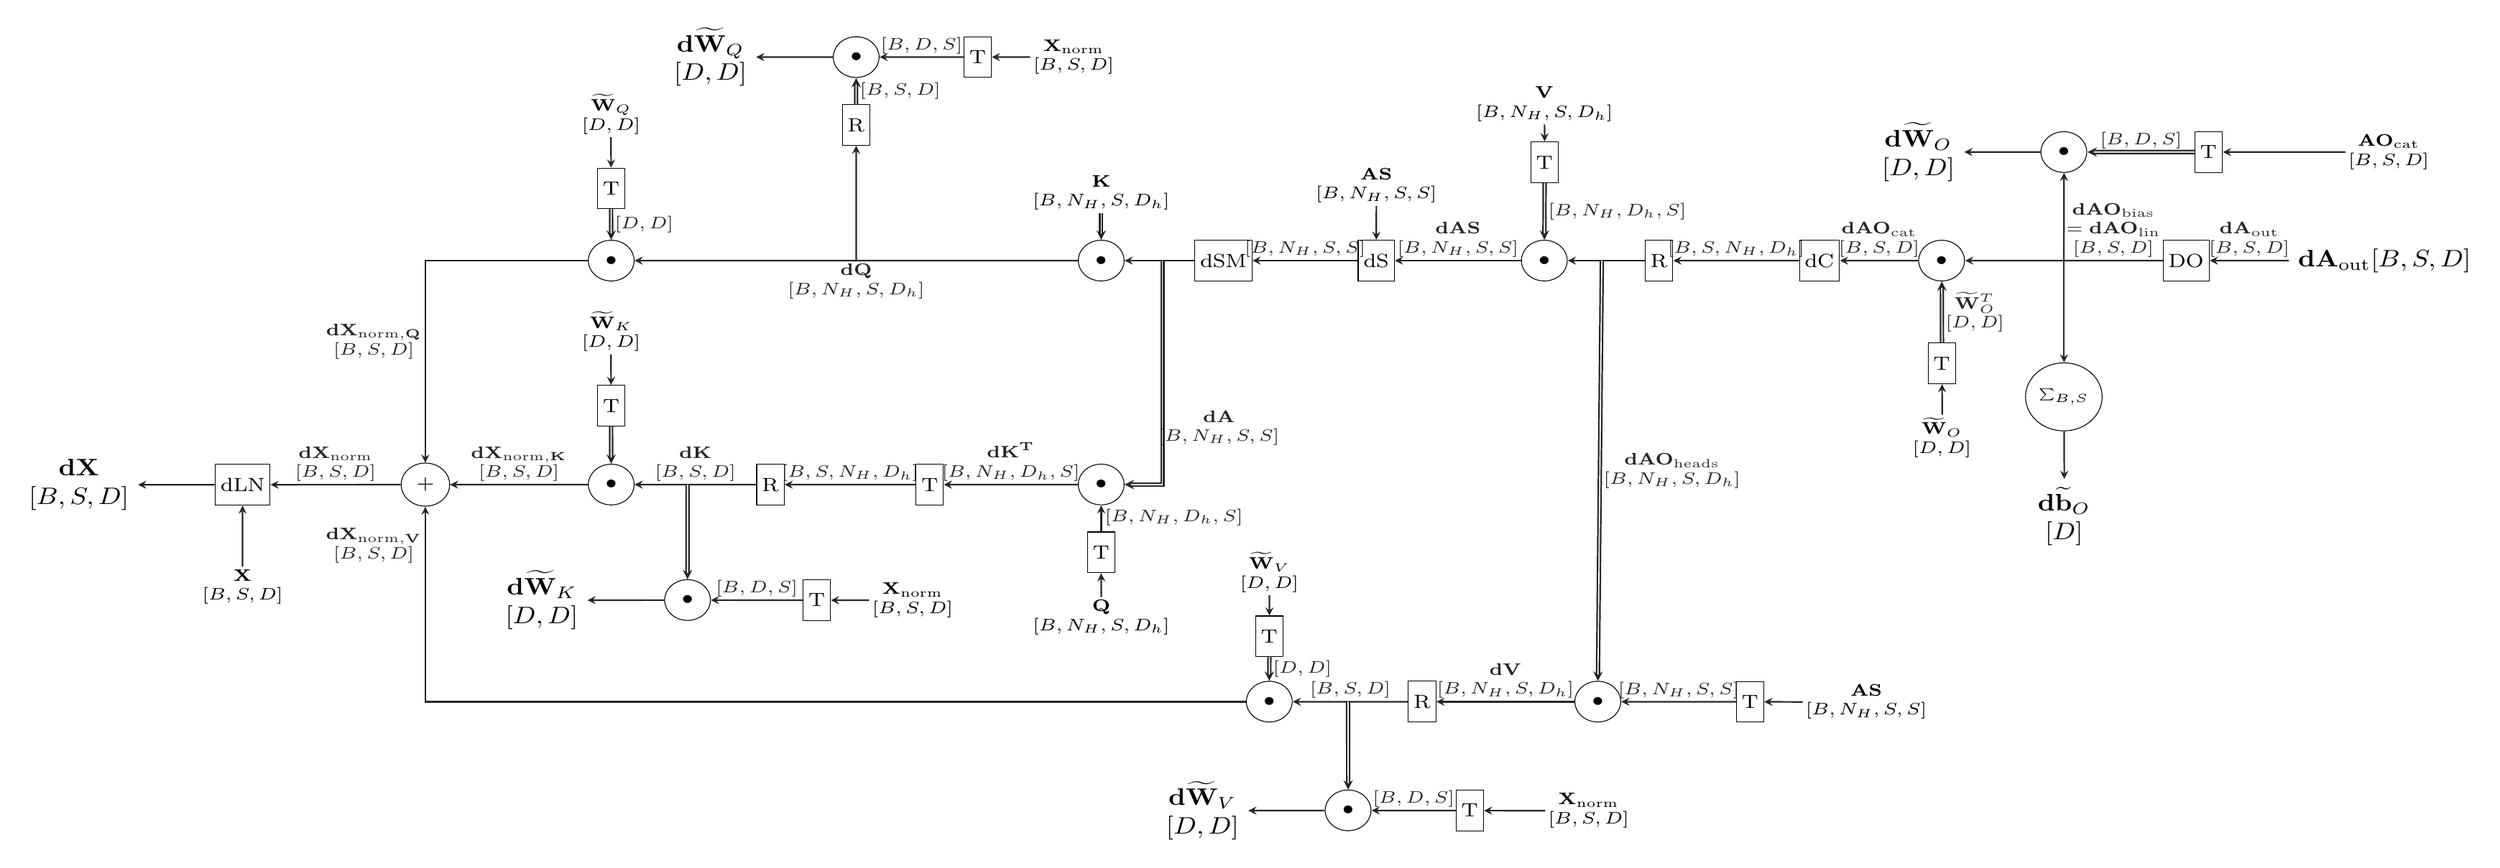
\begin{tikzpicture}[
  every node/.style={transform shape},
  >=stealth,
  auxnode/.style={draw, rectangle, fill=white, minimum height=6mm, inner sep=2pt, font=\footnotesize, align=center},
  mulnode/.style={draw, circle, fill=white, minimum size=6mm, font=\footnotesize, align=center},
  addnode/.style={draw, circle, fill=white, minimum size=6mm, font=\footnotesize, align=center},
  sumnode/.style={draw, circle, fill=white, minimum size=6mm, font=\tiny, align=center},
  flow/.style={->, thick, black!85},
  flow2/.style={->, double, thick, black!85},
  dimlabel/.style={font=\scriptsize, inner sep=1pt, align=center},
  gradflow/.style={->, thick, black!85},
  gradweight/.style={->, thick, black!85}
]

\begin{scope}[xscale=1.35, yscale=1.2]

\def\yoffset{-1.0}
\def\dVXyoffset{-6.5}

\coordinate (Grad_Aout_B) at (17.5, \yoffset);
\coordinate (dDrop_center) at (15.9, \yoffset);
\coordinate (ProjGradSplit) at (14.3, \yoffset);
\coordinate (dOProj_center) at (12.7, \yoffset);
\coordinate (C_center) at (11.1, \yoffset);
\coordinate (R_center) at (9.0, \yoffset);
\coordinate (dPV_AS_calc_center) at (7.5, \yoffset);
\coordinate (dSoft_center) at (5.3, \yoffset);
\coordinate (dSM_calc_center) at (3.3, \yoffset);
\coordinate (dV_calc_center) at (8.2, \dVXyoffset+\yoffset);
\coordinate (R_V_bwd_center) at (5.9, \dVXyoffset+\yoffset);
\coordinate (dVX_calc_center) at (3.9, \dVXyoffset+\yoffset);
\coordinate (dQK_calc_Q_center) at (1.7, \yoffset);
\coordinate (dQK_calc_K_center) at (1.7, -3.3+\yoffset);
\coordinate (K_BWD_input_center) at (1.7, 1.0+\yoffset);
\coordinate (T_Q_bwd_center) at (1.7, -4.3+\yoffset);

% \node[font=\Large\bfseries] at (8, 4.6+\yoffset) {Multi-Head Attention Backward Pass};

\node (Grad_Aout_B) at (18.5, \yoffset) {$\mathbf{dA}_{\text{out}}$\\$[B,S,D]$};
\node[auxnode] (DO) at (dDrop_center) {DO};
\node[mulnode] (dOProj) at (dOProj_center) {$\bullet$};

\node[auxnode] (T_WO) [below=0.9cm of dOProj] {T};
\node[dimlabel] (WO_BWD) [below=0.45cm of T_WO] {$\widetilde{\mathbf{W}}_{O}$\\$[D,D]$};

\node[mulnode] (dWO_calc) at ($(ProjGradSplit)+(0, 1.6)$) {$\bullet$};
\node[align=center, left=1.0cm of dWO_calc]
  (dWO_GRAD) {$\mathbf{d}\widetilde{\mathbf{W}}_{O}$\\$[D,D]$};
\node[auxnode] (T_AO_in) [right=1.4cm of dWO_calc] {T};
\node[dimlabel] (AO_in_local_label) [right=1.6cm of T_AO_in] {$\mathbf{AO}_{\text{cat}}$\\$[B,S,D]$};

\node[auxnode] (C) at (C_center) {dC};
\node[auxnode] (R) at (R_center) {R};

\node[mulnode] (dPV_AS_calc) at (dPV_AS_calc_center) {$\bullet$};
\node[auxnode] (dSoft) at (dSoft_center) {dS};
\node[auxnode] (dSM_calc) at (dSM_calc_center) {dSM};

\node[mulnode] (dQK_calc_Q) at (dQK_calc_Q_center) {$\bullet$};
\node[mulnode] (dQX_proj_calc) [left=5.8cm of dQK_calc_Q] {$\bullet$};

\node[mulnode] (dQK_calc_K) at (dQK_calc_K_center) {$\bullet$};
\node[mulnode] (dKX_proj_calc) [left=5.8cm of dQK_calc_K] {$\bullet$};

\node[dimlabel] (K_BWD_input) at (K_BWD_input_center) {$\mathbf{K}$\\$[B,N_H,S,D_h]$};
\node[auxnode] (T_Q_bwd) at (T_Q_bwd_center) {T};
\node[dimlabel] (Q_BWD_input) [below=0.35cm of T_Q_bwd] {$\mathbf{Q}$\\$[B,N_H,S,D_h]$};

\node[dimlabel] (V_FWD) [above=1.7cm of dPV_AS_calc] {$\mathbf{V}$\\$[B,N_H,S,D_h]$};
\node[auxnode] (T_V_bwd) [below=0.25cm of V_FWD] {T};

\node[mulnode] (dV_calc) at (dV_calc_center) {$\bullet$};
\node[auxnode] (T_AS_bwd) [right=1.5cm of dV_calc] {T};
\node[dimlabel] (AS_BWD_for_V) [right=0.5cm of T_AS_bwd] {$\mathbf{AS}$\\$[B,N_H,S,S]$};

\node[auxnode] (R_V_bwd) at (R_V_bwd_center) {R};
\node[mulnode] (dVX_calc) at (dVX_calc_center) {$\bullet$};

\node[auxnode] (T_WV) [above=0.35cm of dVX_calc] {T};
\node[dimlabel] (WV_BWD) [above=0.3cm of T_WV] {$\widetilde{\mathbf{W}}_{V}$\\$[D,D]$};

\node[sumnode] (Sum_dBO) [below=1.5cm of ProjGradSplit] {$\sum_{B, S}$};
\node (dBO) [align=center, below=0.7cm of Sum_dBO] {$\mathbf{d}\widetilde{\mathbf{b}}_{O}$\\$[D]$};

\draw[gradflow] (Grad_Aout_B) -- (DO)
  node[dimlabel, midway, above]{$\mathbf{dA}_{\text{out}}$\\$[B,S,D]$};

\draw[gradflow] (DO) -- (dOProj)
  node[dimlabel, pos=0.25, above]{$\mathbf{dAO}_{\text{bias}}$\\$=\mathbf{dAO}_{\text{lin}}$\\$[B,S,D]$};

\draw[gradflow] (ProjGradSplit) -- (dWO_calc.south);
\draw[gradflow] (ProjGradSplit) -- ([yshift=-0.75cm]ProjGradSplit) -| (Sum_dBO.north);

\draw[gradflow] (dOProj) -- (C)
  node[dimlabel, midway, above]{$\mathbf{dAO}_{\text{cat}}$\\$[B,S,D]$};
\draw[gradflow] (C) -- (R)
  node[dimlabel, midway, above]{$[B,S,N_H,D_h]$};

\coordinate (R_split_point) at ($(dPV_AS_calc)!0.5!(R)$);
\draw[gradflow] (R.west) -- (dPV_AS_calc.east);
\draw[flow2] (R_split_point) -- (dV_calc.north)
  node[dimlabel, midway, right]{$\mathbf{dAO}_{\text{heads}}$\\$[B,N_H,S,D_h]$};

\draw[gradflow] (V_FWD.south) -- (T_V_bwd.north);
\draw[flow2] (T_V_bwd.south) -- (dPV_AS_calc.north)
  node[dimlabel, midway, right]{$[B,N_H,D_h,S]$};
\draw[gradflow] (dPV_AS_calc.west) -- (dSoft.east)
  node[dimlabel, midway, above]{$\mathbf{dAS}$\\$[B,N_H,S,S]$};

\node (AS_BWD_dS) [dimlabel, above=0.5cm of dSoft] {$\mathbf{AS}$\\$[B,N_H,S,S]$};
\draw[gradflow] (AS_BWD_dS.south) -- (dSoft.north);
\draw[gradflow] (dSoft.west) -- (dSM_calc.east)
  node[dimlabel, midway, above]{$[B,N_H,S,S]$};

\coordinate (dA_Split_X) at ($(dSM_calc_center)!0.5!(dQK_calc_Q_center)$);
\coordinate (dA_Split) at (dA_Split_X |- dQK_calc_Q.east);
\draw[gradflow] (dSM_calc.west) -- (dQK_calc_Q.east);
\draw[flow2] (dA_Split) -- (dA_Split |- dQK_calc_K.east) -- (dQK_calc_K.east)
  node[dimlabel, pos=-1.5, above, yshift=15]{$\mathbf{dA}$\\$[B,N_H,S,S]$};

\draw[flow2] (K_BWD_input.south) -- (dQK_calc_Q.north);
\draw[gradweight] (dQK_calc_Q) -- (dQX_proj_calc)
  node[dimlabel, midway, below]{$\mathbf{dQ}$\\$[B,N_H,S,D_h]$};

\node[auxnode] (T_WQ_bwd) [above=0.45cm of dQX_proj_calc] {T};
\node[dimlabel] (WQ_bwd) [above=0.45cm of T_WQ_bwd] {$\widetilde{\mathbf{W}}_{Q}$\\$[D,D]$};
\draw[flow] (WQ_bwd) -- (T_WQ_bwd);
\draw[flow2] (T_WQ_bwd.south) -- (dQX_proj_calc.north)
  node[dimlabel, midway, right]{$[D,D]$};

\draw[flow] (Q_BWD_input.north) -- (T_Q_bwd.south);
\draw[flow] (T_Q_bwd.north) -- (dQK_calc_K.south)
  node[dimlabel, pos=0.55, right]{$[B,N_H,D_h,S]$};

\node[auxnode] (T_dK) at ($(dQK_calc_K)!0.35!(dKX_proj_calc)$) {T};
\node[auxnode] (R_dK_mid) at ($(T_dK)!0.5!(dKX_proj_calc)$) {R};

\draw[gradweight] (dQK_calc_K) -- (T_dK)
  node[dimlabel, midway, above]{$\mathbf{dK^T}$\\$[B,N_H,D_h,S]$};
\draw[gradweight] (T_dK) -- (R_dK_mid)
  node[dimlabel, midway, above]{$[B,S,N_H,D_h]$};
\draw[gradweight] (R_dK_mid) -- (dKX_proj_calc)
  node[dimlabel, midway, above]{$\mathbf{dK}$\\$[B,S,D]$};

\node[auxnode] (T_WK_bwd) [above=0.55cm of dKX_proj_calc] {T};
\node[dimlabel] (WK_bwd) [above=0.45cm of T_WK_bwd] {$\widetilde{\mathbf{W}}_{K}$\\$[D,D]$};
\draw[gradflow] (WK_bwd) -- (T_WK_bwd);
\draw[flow2] (T_WK_bwd.south) -- (dKX_proj_calc.north);

\draw[gradflow] (AS_BWD_for_V.west) -- (T_AS_bwd.east);
\draw[gradflow] (T_AS_bwd.west) -- (dV_calc.east)
  node[dimlabel, midway, above]{$[B,N_H,S,S]$};
\draw[gradflow] (dV_calc.west) -- (R_V_bwd.east)
  node[dimlabel, midway, above]{$\mathbf{dV}$\\$[B,N_H,S,D_h]$};
\draw[gradflow] (R_V_bwd) -- (dVX_calc.east)
  node[dimlabel, midway, above]{$[B,S,D]$};

\draw[gradflow] (WV_BWD) -- (T_WV);
\draw[flow2] (T_WV) -- (dVX_calc.north)
  node[dimlabel, midway, right]{$[D,D]$};

\node[addnode] (Sum_dXnorm) [left=1.8cm of dKX_proj_calc] {$+$};

\draw[gradweight] (dQX_proj_calc.west) -| node[dimlabel, pos=0.7, left]{$\mathbf{dX}_{\text{norm},\mathbf{Q}}$\\$[B,S,D]$} (Sum_dXnorm.north);
\draw[gradweight] (dKX_proj_calc.west) -- node[dimlabel, midway, above]{$\mathbf{dX}_{\text{norm},\mathbf{K}}$\\$[B,S,D]$} (Sum_dXnorm.east);
\draw[gradweight] (dVX_calc.west) -| node[dimlabel, pos=0.9, left]{$\mathbf{dX}_{\text{norm},\mathbf{V}}$\\$[B,S,D]$} (Sum_dXnorm.south);

\coordinate (dV_branch) at ($(R_V_bwd.west)!0.52!(dVX_calc.east)$);
\node[mulnode] (dWV_mul) at ($(dV_branch)+(0,-1.6cm)$) {$\bullet$};
\draw[flow2] (dV_branch) -- (dWV_mul.north);

\node[auxnode] (T_Xnorm) [right=1.1cm of dWV_mul] {T};
\node[dimlabel] (Xnorm_local) [right=0.8cm of T_Xnorm] {$\mathbf{X}_{\text{norm}}$\\$[B,S,D]$};
\draw[gradflow] (Xnorm_local) -- (T_Xnorm);
\draw[gradflow] (T_Xnorm.west) -- (dWV_mul.east)
  node[dimlabel, midway, above]{$[B,D,S]$};
\node (dWV_out) [align=center, left=1.0cm of dWV_mul] {$\mathbf{d}\widetilde{\mathbf{W}}_{V}$\\$[D,D]$};
\draw[gradweight] (dWV_mul.west) -- (dWV_out);

\coordinate (dQ_branch) at ($(dQK_calc_Q.east)!0.50!(dQX_proj_calc.west)$);
\node[mulnode] (dWQ_mul) at ($(dQ_branch)+(0,3.0cm)$) {$\bullet$};
\node[auxnode] (R_dQ_for_WQ) at ($(dWQ_mul)+(0,-1.0cm)$) {R};
\draw[gradflow]  (dQ_branch) -- (R_dQ_for_WQ.south);
\draw[flow2] (R_dQ_for_WQ.north) -- (dWQ_mul.south)
  node[dimlabel, midway, right]{$[B,S,D]$};

\node[auxnode] (T_XnormQ) [right=1.1cm of dWQ_mul] {T};
\node[dimlabel] (Xnorm_localQ) [right=0.5cm of T_XnormQ] {$\mathbf{X}_{\text{norm}}$\\$[B,S,D]$};
\draw[gradflow] (Xnorm_localQ) -- (T_XnormQ);
\draw[gradflow] (T_XnormQ.west) -- (dWQ_mul.east)
  node[dimlabel, midway, above]{$[B,D,S]$};
\node (dWQ_out) [align=center, left=1.0cm of dWQ_mul] {$\mathbf{d}\widetilde{\mathbf{W}}_{Q}$\\$[D,D]$};
\draw[gradweight] (dWQ_mul.west) -- (dWQ_out);

\coordinate (dK_branch) at ($(R_dK_mid)!0.52!(dKX_proj_calc)$);
\node[mulnode] (dWK_mul) at ($(dK_branch)+(0,-1.7cm)$) {$\bullet$};
\draw[flow2]  (dK_branch) -- (dWK_mul.north);

\node[auxnode] (T_XnormK) [right=1.2cm of dWK_mul] {T};
\node[dimlabel, right=0.5cm of T_XnormK] (Xnorm_localK) {$\mathbf{X}_{\text{norm}}$\\$[B,S,D]$};
\draw[gradflow] (Xnorm_localK) -- (T_XnormK);
\draw[gradflow] (T_XnormK.west) -- (dWK_mul.east)
  node[dimlabel, midway, above]{$[B,D,S]$};
\node (dWK_out) [align=center, left=1.0cm of dWK_mul] {$\mathbf{d}\widetilde{\mathbf{W}}_{K}$\\$[D,D]$};
\draw[gradweight] (dWK_mul.west) -- (dWK_out);

\draw[gradweight] (Sum_dBO) -- (dBO);

\draw[gradflow] (WO_BWD) -- (T_WO);
\draw[flow2] (T_WO) -- (dOProj)
  node[dimlabel, midway, right]{$\widetilde{\mathbf{W}}_{O}^{T}$\\$[D,D]$};
\draw[gradflow] (AO_in_local_label) -- (T_AO_in);
\draw[flow2] (T_AO_in) -- (dWO_calc.east)
  node[dimlabel, midway, above]{$[B,D,S]$};
\draw[gradweight] (dWO_calc) -- (dWO_GRAD);

\node[auxnode] (dLN) [left=1.7cm of Sum_dXnorm] {dLN};
\draw[gradweight] (Sum_dXnorm.west) -- node[dimlabel, midway, above]
  {$\mathbf{dX}_{\text{norm}}$\\$[B,S,D]$} (dLN.east);

\node (dX_OUT) [align=center, left=1.0cm of dLN] {$\mathbf{dX}$\\$[B,S,D]$};
\draw[gradweight] (dLN.west) -- (dX_OUT);

\node[dimlabel] (LNCache) [below=0.9cm of dLN] {$\mathbf{X}$\\$[B,S,D]$};
\draw[gradflow] (LNCache.north) -- (dLN.south);

\end{scope}
\end{tikzpicture}
}

  \caption{단일 노드 MHA 블록의 역전파.
  출력 $\mathbf{A}_{\text{out}}$에 대한 기울기에서 시작하여,
  출력 프로젝션, 어텐션 연산, Q/K/V 선형 레이어, 레이어 정규화를
  역순으로 거치며 입력과 파라미터에 대한 기울기를 계산한다.}
  \label{fig:single_node_mha_backward}
\end{figure}
\end{landscape}


% ------------------------ 5.3 MLP / FFN ------------------------------

\subsection{피드포워드 네트워크 (MLP / FFN)}

트랜스포머 블록의 MLP(또는 FFN) 부분은
각 시퀀스 위치별로 독립적인 비선형 변환을 수행한다.
구조적으로는 두 개의 선형 레이어와 중간 비선형 함수로 이루어져 있으며,
앞에서 정의한
\[
  \mathbf{X}, \mathbf{Y} \in \mathbb{R}^{B \times S \times D}, \quad
  \mathbf{Z}_{\text{up}}, \mathbf{Z}_{\text{act}}
  \in \mathbb{R}^{B \times S \times D_{\text{ff}}}
\]
를 사용한다.

\subsubsection{순전파}

MHA 블록의 출력을 $\mathbf{A}_{\text{out}}$라 두고,
잔차 연결까지 반영된 텐서를 $\mathbf{X}_2$라고 하자
(Section~\ref{sec:background}의 트랜스포머 블록 구조 참조).
MLP 블록에서는 다음과 같은 순서를 따른다.

\paragraph{(1) 레이어 정규화.}
\[
  \mathbf{X}_3 = \mathrm{LN}(\mathbf{X}_2)
  \in \mathbb{R}^{B \times S \times D}.
\]

\paragraph{(2) 상향 선형 레이어 (up-projection).}
\[
  \mathbf{Z}_{\text{up}} = \mathbf{X}_3 W_{\text{up}} + \mathbf{b}_{\text{up}},
\]
여기서 $W_{\text{up}} \in \mathbb{R}^{D \times D_{\text{ff}}}$,
$\mathbf{b}_{\text{up}} \in \mathbb{R}^{D_{\text{ff}}}$이다.

\paragraph{(3) 비선형 활성 함수.}
\[
  \mathbf{Z}_{\text{act}} = \phi(\mathbf{Z}_{\text{up}}),
\]
GELU, ReLU 등 원소별 비선형 함수를 사용한다.

\paragraph{(4) 하향 선형 레이어 (down-projection).}
\[
  \mathbf{H}_{\text{mlp}}
  = \mathbf{Z}_{\text{act}} W_{\text{down}} + \mathbf{b}_{\text{down}},
\]
여기서 $W_{\text{down}} \in \mathbb{R}^{D_{\text{ff}} \times D}$,
$\mathbf{b}_{\text{down}} \in \mathbb{R}^{D}$이다.

\paragraph{(5) 잔차 연결.}
최종적으로 MLP 출력은
\[
  \mathbf{X}_{\text{out}} = \mathbf{X}_2 + \mathbf{H}_{\text{mlp}}
\]
와 같이 잔차 연결을 통해 합쳐진다.

\begin{figure}[htbp]
  \centering
  \resizebox{\linewidth}{!}{%
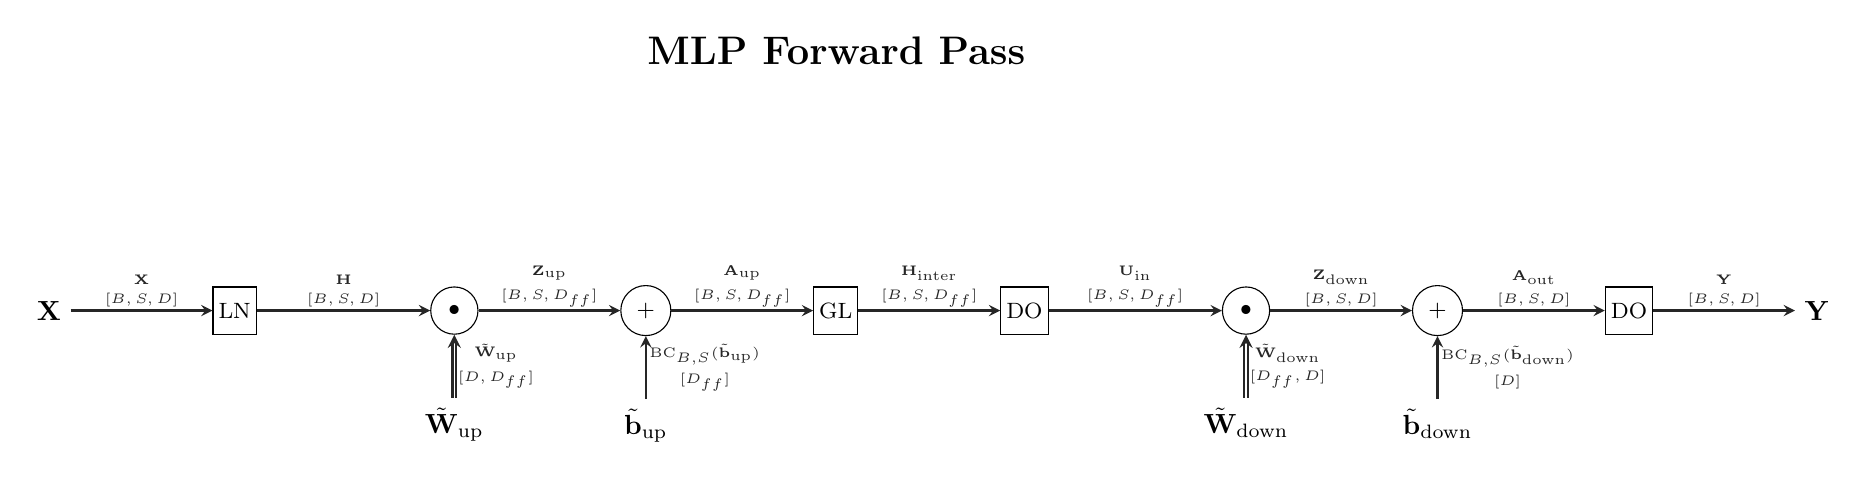
\begin{tikzpicture}[
    >=stealth,
    auxnode/.style={draw, rectangle, fill=white, minimum height=6mm, inner sep=2pt, font=\footnotesize, align=center},
    mulnode/.style={draw, circle, fill=white, minimum size=6mm, font=\footnotesize, align=center},
    addnode/.style={draw, circle, fill=white, minimum size=6mm, font=\footnotesize, align=center},
    sumnode/.style={draw, circle, fill=white, minimum size=6mm, font=\tiny, align=center},
    flow/.style={->, thick, black!85},
    flow2/.style={double, ->, thick, black!85},
    dimlabel/.style={font=\tiny, inner sep=1pt, align=center}
]
    \node[font=\Large\bfseries] at (10, 2.8) {MLP Forward Pass};

    \pgfmathsetmacro{\verticaloffset}{-0.5}

    \node            (MIn)   at (0,\verticaloffset) {$\mathbf{X}$};
    \node[auxnode]   (LN2)   [right=1.8cm of MIn] {LN};
    \node[mulnode]   (L1Mul) [right=2.2cm of LN2] {$\bullet$};
    \node            (Wup)   [below=0.8cm of L1Mul] {$\tilde{\mathbf{W}}_{\text{up}}$};
    \node[addnode]   (AddB1) [right=1.8cm of L1Mul] {+};
    \node            (Bup)   [below=0.8cm of AddB1] {$\tilde{\mathbf{b}}_{\text{up}}$};
    \node[auxnode]   (Act)   [right=1.8cm of AddB1] {GL};
    \node[auxnode]   (Drop1) [right=1.8cm of Act] {DO};
    \node[mulnode]   (L2Mul) [right=2.2cm of Drop1] {$\bullet$};
    \node            (Wdown) [below=0.8cm of L2Mul] {$\tilde{\mathbf{W}}_{\text{down}}$};
    \node[addnode]   (AddB2) [right=1.8cm of L2Mul] {+};
    \node            (Bdown) [below=0.8cm of AddB2] {$\tilde{\mathbf{b}}_{\text{down}}$};
    \node[auxnode]   (Drop2) [right=1.8cm of AddB2] {DO};
    \node            (MOut)  [right=1.8cm of Drop2] {$\mathbf{Y}$};

    \draw[flow] (MIn) -- (LN2) node[dimlabel, midway, above]{\shortstack{$\mathbf{X}$\\$[B,S,D]$}};
    \draw[flow] (LN2) -- (L1Mul) node[dimlabel, midway, above]{\shortstack{$\mathbf{H}$\\$[B,S,D]$}};
    \draw[flow2] (Wup) -- (L1Mul) node[dimlabel, midway, right]{\shortstack{$\tilde{\mathbf{W}}_{\text{up}}$\\$[D, D_{ff}]$}};
    \draw[flow] (L1Mul) -- (AddB1) node[dimlabel, midway, above]{\shortstack{$\mathbf{Z}_{\text{up}}$\\$[B,S,D_{ff}]$}};
    \draw[flow] (Bup) -- (AddB1) node[dimlabel, midway, right]{\shortstack{$\mathrm{BC}_{B,S}(\tilde{\mathbf{b}}_{\text{up}})$\\$[D_{ff}]$}};
    \draw[flow] (AddB1) -- (Act) node[dimlabel, midway, above]{\shortstack{$\mathbf{A}_{\text{up}}$\\$[B,S,D_{ff}]$}};
    \draw[flow] (Act) -- (Drop1) node[dimlabel, midway, above]{\shortstack{$\mathbf{H}_{\text{inter}}$\\$[B,S,D_{ff}]$}};
    \draw[flow] (Drop1) -- (L2Mul) node[dimlabel, midway, above]{\shortstack{$\mathbf{U}_{\text{in}}$\\$[B,S,D_{ff}]$}};
    \draw[flow2] (Wdown) -- (L2Mul) node[dimlabel, midway, right]{\shortstack{$\tilde{\mathbf{W}}_{\text{down}}$\\$[D_{ff}, D]$}};
    \draw[flow] (L2Mul) -- (AddB2) node[dimlabel, midway, above]{\shortstack{$\mathbf{Z}_{\text{down}}$\\$[B,S,D]$}};
    \draw[flow] (Bdown) -- (AddB2) node[dimlabel, midway, right]{\shortstack{$\mathrm{BC}_{B,S}(\tilde{\mathbf{b}}_{\text{down}})$\\$[D]$}};
    \draw[flow] (AddB2) -- (Drop2) node[dimlabel, midway, above]{\shortstack{$\mathbf{A}_{\text{out}}$\\$[B,S,D]$}};
    \draw[flow] (Drop2) -- (MOut) node[dimlabel, midway, above]{\shortstack{$\mathbf{Y}$\\$[B,S,D]$}};

\end{tikzpicture}%
}

  \caption{단일 노드 MLP/FFN 블록의 순전파.
  입력 $\mathbf{X}_2$는 레이어 정규화를 거쳐 상향 선형 레이어,
  비선형 활성 함수, 하향 선형 레이어를 통과한 뒤,
  잔차 연결을 통해 $\mathbf{X}_{\text{out}}$을 형성한다.}
  \label{fig:single_node_mlp_forward}
\end{figure}

\subsubsection{역전파}

역전파에서는 $\mathrm{d}\mathbf{X}_{\text{out}}$에서 시작하여
잔차 연결을 통해 $\mathrm{d}\mathbf{X}_2$와
$\mathrm{d}\mathbf{H}_{\text{mlp}}$를 얻고,
이후 각 선형 레이어와 비선형 함수, 레이어 정규화를
역순으로 따라가며 기울기를 계산한다.

구체적으로는 다음과 같은 단계로 이해할 수 있다.
\begin{itemize}
  \item 잔차 연결 역전파: $\mathrm{d}\mathbf{X}_2$와
        $\mathrm{d}\mathbf{H}_{\text{mlp}}$가 동일한 기울기를 받는다.
  \item 하향 선형 레이어 역전파를 통해
        $\mathrm{d}\mathbf{Z}_{\text{act}}$, $W_{\text{down}}$과
        $\mathbf{b}_{\text{down}}$에 대한 기울기를 계산한다.
  \item 비선형 함수 역전파를 통해 $\mathrm{d}\mathbf{Z}_{\text{up}}$를 얻는다.
  \item 상향 선형 레이어 역전파를 통해
        $\mathrm{d}\mathbf{X}_3$, $W_{\text{up}}$과
        $\mathbf{b}_{\text{up}}$에 대한 기울기를 계산한다.
  \item 마지막으로 레이어 정규화 역전파를 통해
        $\mathrm{d}\mathbf{X}_2$를 입력 방향으로 전파한다.
\end{itemize}

\begin{figure}[htbp]
  \centering
  \noindent
\resizebox{\linewidth}{!}{%
\begin{tikzpicture}[
    >=stealth,
    auxnode/.style={draw, rectangle, fill=white, minimum height=6mm, inner sep=2pt, font=\footnotesize, align=center},
    mulnode/.style={draw, circle, fill=white, minimum size=6mm, font=\footnotesize, align=center},
    addnode/.style={draw, circle, fill=white, minimum size=6mm, font=\footnotesize, align=center},
    sumnode/.style={draw, circle, fill=white, minimum size=6mm, font=\tiny, align=center},
    flow_rev/.style={<-, thick, black!85},
    flow_dw/.style={->, thick, black!85},
    flow_act/.style={double, ->, thick, black!85},
    dimlabel/.style={font=\tiny, inner sep=1pt, align=center},
    gradlabel/.style={font=\tiny\bfseries, inner sep=1pt, align=center}
]
    \node[font=\Large\bfseries] at (5, 10) {MLP Backward Pass};

    \pgfmathsetmacro{\backwardoffset}{0.0}

    \node (d_MOut) at (12.6, \backwardoffset) {$\mathrm{d}\mathbf{Y}$};
    \node[auxnode] (d_Drop2) [left=1.8cm of d_MOut] {dDO};
    \draw[flow_rev] (d_Drop2) -- (d_MOut)
      node[dimlabel, midway, below]{\shortstack{$\mathrm{d}\mathbf{Y}$\\$[B,S,D]$}};

    \coordinate (split2) at ($(d_Drop2.west) + (-1.5cm, 0)$);
    \coordinate (branch_dUproj) at ($(split2) + (-1.2cm, 0)$);

    \node[sumnode] (d_SumB2) [above=0.8cm of split2] {$\sum_{B, S}$};
    \node (d_Bdown) [above=0.8cm of d_SumB2] {$\mathrm{d}\tilde{\mathbf{b}}_{\text{down}}$};
    \draw[flow_dw] (d_SumB2) -- (d_Bdown) node[dimlabel, midway, right]{$[D]$};

    \draw[flow_rev] (split2) -- (d_Drop2);
    \draw[flow_rev] (d_SumB2) -- (split2);

    \node[mulnode] (d_L2Mul_in) [left=2.2cm of split2] {$\bullet$};
    \draw[flow_rev] (d_L2Mul_in) -- (d_Drop2)
      node[gradlabel, midway, below]{\shortstack{$\mathrm{d}\mathbf{Z}_{\text{down}}=\mathrm{d}\mathbf{A}_{\text{out}}$\\$[B,S,D]$}};

    \node (W_down_T) [below=1.8cm of d_L2Mul_in] {$\tilde{\mathbf{W}}_{\text{down}}^{T}$};
    \draw[flow_act] (W_down_T.north) -- (d_L2Mul_in)
      node[dimlabel, midway, right]{$[D, D_{ff}]$};

    \coordinate (L2Mul_w_y) at ($(d_L2Mul_in) + (0, 3.5cm)$);
    \node[mulnode] (d_L2Mul_w) at (L2Mul_w_y) {$\bullet$};
    \node (d_Wdown) [above=0.8cm of d_L2Mul_w] {$\mathrm{d}\tilde{\mathbf{W}}_{\text{down}}$};
    \draw[flow_dw] (d_L2Mul_w) -- (d_Wdown) node[dimlabel, midway, right]{$[D_{ff}, D]$};

    \draw[flow_act] (branch_dUproj.north) |- (d_L2Mul_w.east);

    \node[auxnode] (Uin_T) at ($(d_L2Mul_w.west) + (-1.5cm, 0)$) {T};
    \draw[flow_dw] (Uin_T) -- (d_L2Mul_w)
      node[dimlabel, midway, below]{\shortstack{$\mathbf{U}_{\text{in}}^T$\\$[B, D_{ff}, S]$}};
    \node (Uin_aux) [left=1.8cm of Uin_T] {$\mathbf{U}_{\text{in}}$};
    \draw[flow_dw] (Uin_aux) -- (Uin_T) node[dimlabel, midway, above]{\shortstack{$[B,S,D_{ff}]$}};

    \node[auxnode] (d_Drop1) [left=1.8cm of d_L2Mul_in] {dDO};
    \draw[flow_rev] (d_Drop1) -- (d_L2Mul_in)
      node[dimlabel, midway, below]{\shortstack{$\mathrm{d}\mathbf{U}_{\text{in}}$\\$[B,S,D_{ff}]$}};

    \node[auxnode] (d_Act) [left=1.8cm of d_Drop1] {dGL};
    \draw[flow_rev] (d_Act) -- (d_Drop1)
      node[dimlabel, midway, below]{\shortstack{$\mathrm{d}\mathbf{H}_{\text{inter}}$\\$[B,S,D_{ff}]$}};

    \coordinate (split1) at ($(d_Act.west) + (-1.5cm, 0)$);
    \coordinate (branch_dHpre) at ($(split1) + (-1.2cm, 0)$);

    \node[sumnode] (d_SumB1) [above=0.8cm of split1] {$\sum_{B, S}$};
    \node (d_Bup) [above=0.8cm of d_SumB1] {$\mathrm{d}\tilde{\mathbf{b}}_{\text{up}}$};
    \draw[flow_dw] (d_SumB1) -- (d_Bup) node[dimlabel, midway, right]{$[D_{ff}]$};

    \draw[flow_rev] (split1) -- (d_Act);
    \draw[flow_rev] (d_SumB1) -- (split1);

    \node[mulnode] (d_L1Mul_in) [left=2.2cm of split1] {$\bullet$};
    \draw[flow_rev] (d_L1Mul_in) -- (d_Act)
      node[gradlabel, midway, below]{\shortstack{$\mathrm{d}\mathbf{Z}_{\text{up}}=\mathrm{d}\mathbf{A}_{\text{up}}$\\$[B,S,D_{ff}]$}};

    \node (W_up_T) [below=1.8cm of d_L1Mul_in] {$\tilde{\mathbf{W}}_{\text{up}}^{T}$};
    \draw[flow_act] (W_up_T.north) -- (d_L1Mul_in)
      node[dimlabel, midway, right]{$[D_{ff}, D]$};

    \coordinate (L1Mul_w_y) at ($(d_L1Mul_in) + (0, 3.5cm)$);
    \node[mulnode] (d_L1Mul_w) at (L1Mul_w_y) {$\bullet$};
    \node (d_Wup) [above=0.8cm of d_L1Mul_w] {$\mathrm{d}\tilde{\mathbf{W}}_{\text{up}}$};
    \draw[flow_dw] (d_L1Mul_w) -- (d_Wup) node[dimlabel, midway, right]{$[D, D_{ff}]$};

    \draw[flow_act] (branch_dHpre.north) |- (d_L1Mul_w.east);

    \node[auxnode] (Znorm_T) at ($(d_L1Mul_w.west) + (-1.5cm, 0)$) {T};
    \draw[flow_dw] (Znorm_T) -- (d_L1Mul_w)
      node[dimlabel, midway, below]{\shortstack{$\mathbf{H}^T$\\$[B, D, S]$}};
    \node (Znorm_aux) [left=1.8cm of Znorm_T] {$\mathbf{H}$};
    \draw[flow_dw] (Znorm_aux) -- (Znorm_T) node[dimlabel, midway, above]{\shortstack{$[B,S,D]$}};

    \node[auxnode] (d_LN2) [left=1.8cm of d_L1Mul_in] {dLN};
    \draw[flow_rev] (d_LN2) -- (d_L1Mul_in)
      node[dimlabel, midway, below]{\shortstack{$\mathrm{d}\mathbf{H}$\\$[B,S,D]$}};

    \node (d_MIn) [left=1.8cm of d_LN2] {$\mathrm{d}\mathbf{X}$};
    \draw[flow_rev] (d_MIn) -- (d_LN2)
      node[dimlabel, midway, below]{\shortstack{$\mathrm{d}\mathbf{X}$\\$[B,S,D]$}};
\end{tikzpicture}%
}

  \caption{단일 노드 MLP/FFN 블록의 역전파.
  잔차 연결, 하향/상향 선형 레이어, 비선형 함수, 레이어 정규화를
  역순으로 통과하며, 각 입력과 파라미터에 대한 기울기를 계산한다.}
  \label{fig:single_node_mlp_backward}
\end{figure}


% ------------------------ 5.4 Output Projection and Loss -------------

\subsection{출력 프로젝션과 손실}

마지막으로, 트랜스포머 레이어의 출력
$\mathbf{X}_{\text{out}} \in \mathbb{R}^{B \times S \times D}$에서
언어 모델 로그릿(logits)을 만들고, 손실을 계산하는 부분을 살펴본다.
여기서는 언어 모델링 또는 다음 토큰 예측을 위한
전형적인 설정을 가정한다.

출력 프로젝션은 언어 모델 행렬 $W_{\text{lm}} \in \mathbb{R}^{D \times V}$
및 bias $\mathbf{b}_{\text{lm}} \in \mathbb{R}^{V}$를 사용하여,
각 위치마다 어휘 크기 $V$에 대한 로그릿을 생성한다.
\[
  \mathbf{Z}_{\text{lm}}[b,s,:]
  = \mathbf{X}_{\text{out}}[b,s,:]\, W_{\text{lm}} + \mathbf{b}_{\text{lm}}.
\]
손실은 보통 소프트맥스-교차 엔트로피(softmax-cross-entropy)로 정의된다.

\subsubsection{순전파 (로그릿, 소프트맥스, 손실)}

순전파는 개념적으로 다음과 같은 단계를 따른다.
\begin{itemize}
  \item $\mathbf{X}_{\text{out}}$에 선형 레이어를 적용하여
        로그릿 텐서 $\mathbf{Z}_{\text{lm}} \in \mathbb{R}^{B \times S \times V}$를 얻는다.
  \item 각 위치별로 소프트맥스를 적용하여 확률 분포를 계산한다.
  \item 목표 토큰(예: 다음 토큰)의 원-핫(one-hot) 벡터와 로그릿을 사용해
        교차 엔트로피 손실을 계산하고, 전체 배치/시퀀스에 대해 평균(또는 합)을 취한다.
\end{itemize}

\begin{figure}[htbp]
  \centering
  
\noindent
\resizebox{\linewidth}{!}{%
\begin{tikzpicture}[
  >=stealth,
  auxnode/.style={draw, rectangle, fill=white, minimum height=6mm, inner sep=2pt, font=\footnotesize, align=center},
  mulnode/.style={draw, circle, fill=white, minimum size=6mm, font=\footnotesize, align=center},
  addnode/.style={draw, circle, fill=white, minimum size=6mm, font=\footnotesize, align=center},
  sumnode/.style={draw, circle, fill=white, minimum size=6mm, font=\tiny, align=center},
  flow/.style={->, thick, black!85},
  flow2/.style={double, ->, thick, black!85},
  dimlabel/.style={font=\tiny, inner sep=1pt, align=center}
]

% From Transformer output
\node            (H)     at (0,-2) {$\mathbf{A}_{\text{out}}$};

% LM head
\node[mulnode]   (LMmul) [right=2.2cm of H] {$\bullet$};
\node            (Wlm)   [align=center, below=0.9cm of LMmul] {$\widetilde{\mathbf{W}}_{\text{lm}}$\\$=\mathbf{E}^{T}$};
\node[addnode]   (AddB)  [right=1.8cm of LMmul] {+};
\node            (blm)   [below=0.9cm of AddB] {$\widetilde{\mathbf{b}}_{\text{lm}}$};

% Softmax → Prob
\node[auxnode]   (SM)    [right=1.8cm of AddB] {S};

\node[auxnode] (ARG)  [right=4.0cm of SM] {ARG};
% Midpoint of SM→P edge (for CE tap)
\coordinate (MidSP) at ($(SM)!0.5!(ARG)$);

% CE node placed below the SM→P edge
\node[auxnode]   (CE)    [below=1.6cm of MidSP] {CE};
\node            (Y)     [right=0.9cm of CE] {$\mathbf{Y_\text{targets}}$};
\node            (Loss)  [align=center, below=1.8cm of CE] {$\mathcal{L}$\\ (mean over $B,S$)};

% Flows
\draw[flow]  (H) -- (LMmul) node[dimlabel, midway, above]{\shortstack{$[B,S,D]$}};
\draw[flow2] (Wlm) -- (LMmul) node[dimlabel, midway, right]{\shortstack{$[D,V]$}};
\draw[flow]  (LMmul) -- (AddB) node[dimlabel, midway, above]{\shortstack{$\mathbf{Z}_{\text{lin}}$\\$[B,S,V]$}};
\draw[flow]  (blm) -- (AddB)   node[dimlabel, midway, right]{\shortstack{$\text{BC}_{B,S}(\widetilde{\mathbf{b}}_{\text{lm}})$\\$[V]$}};
\draw[flow]  (AddB) -- (SM)    node[dimlabel, midway, above]{\shortstack{\textbf{Z\textsubscript{bias}}\\ $[B,S,V]$}};

% Tap the SM→P edge downward into CE
\draw[flow]  (MidSP) -- (CE);
% Targets into CE
\draw[flow]  (Y) -- (CE)  node[dimlabel, midway, above]{\shortstack{targets\\$[B,S]$}};
% Loss goes WEST (left) from CE
\draw[flow]  (CE) -- (Loss);

\node (YhatG) [right=1.8cm of ARG] {$\hat{\mathbf{Y}}_{\text{greedy}}$};
\draw[flow] (SM) -- (ARG)
  node[dimlabel, pos=0.35, above]{\shortstack{$\mathbf{P}$\\$[B,S,V]$}};
\draw[flow] (ARG) -- (YhatG)
  node[dimlabel, midway, above]{\shortstack{token ids\\$[B,S]$}};

% Optional: top-k (or nucleus) sampling path
\node[auxnode] (TopK) [above=1.4cm of ARG] {TOP-$k$};
\node          (YhatS) [right=1.8cm of TopK] {$\hat{\mathbf{Y}}_{\text{sample}}$};
\draw[flow] (MidSP) |- (TopK);
\draw[flow] (TopK) -- (YhatS)
  node[dimlabel, midway, above]{\shortstack{token ids\\$[B,S]$}};

\node[font=\large\bfseries] at (9.2,1.8) {Token Generation \& Loss (Forward)};
\end{tikzpicture}%
}

  \caption{출력 프로젝션과 손실의 순전파.
  은닉 상태 $\mathbf{X}_{\text{out}}$는 언어 모델 프로젝션
  $(W_{\text{lm}}, \mathbf{b}_{\text{lm}})$을 통해 로그릿으로 변환되고,
  소프트맥스와 교차 엔트로피를 거쳐 스칼라 손실 $\mathcal{L}$이 계산된다.}
  \label{fig:single_node_output_forward}
\end{figure}

\subsubsection{역전파}

역전파에서는 손실 $\mathcal{L}$로부터 시작하여,
소프트맥스와 교차 엔트로피를 통합한 형태의 기울기가
로그릿 $\mathbf{Z}_{\text{lm}}$에 대해 계산된다.
실제로는 소프트맥스와 교차 엔트로피의 역전파가 하나의
간단한 표현으로 합쳐지는 경우가 많다.

그 다음 단계는 다음과 같다.
\begin{itemize}
  \item 로그릿에 대한 기울기 $\mathrm{d}\mathbf{Z}_{\text{lm}}$를
        출력 프로젝션 선형 레이어를 통해 역전파하여,
        $\mathrm{d}\mathbf{X}_{\text{out}}$와
        $\mathrm{d}W_{\text{lm}}, \mathrm{d}\mathbf{b}_{\text{lm}}$을 얻는다.
  \item $\mathrm{d}\mathbf{X}_{\text{out}}$는 다시 이전 MLP/FFN 블록과
        MHA, 임베딩 레이어로 전달된다
        (Figure~\ref{fig:single_node_overall} 참고).
\end{itemize}

\begin{figure}[htbp]
  \centering
  \noindent
\resizebox{0.8\linewidth}{!}{%
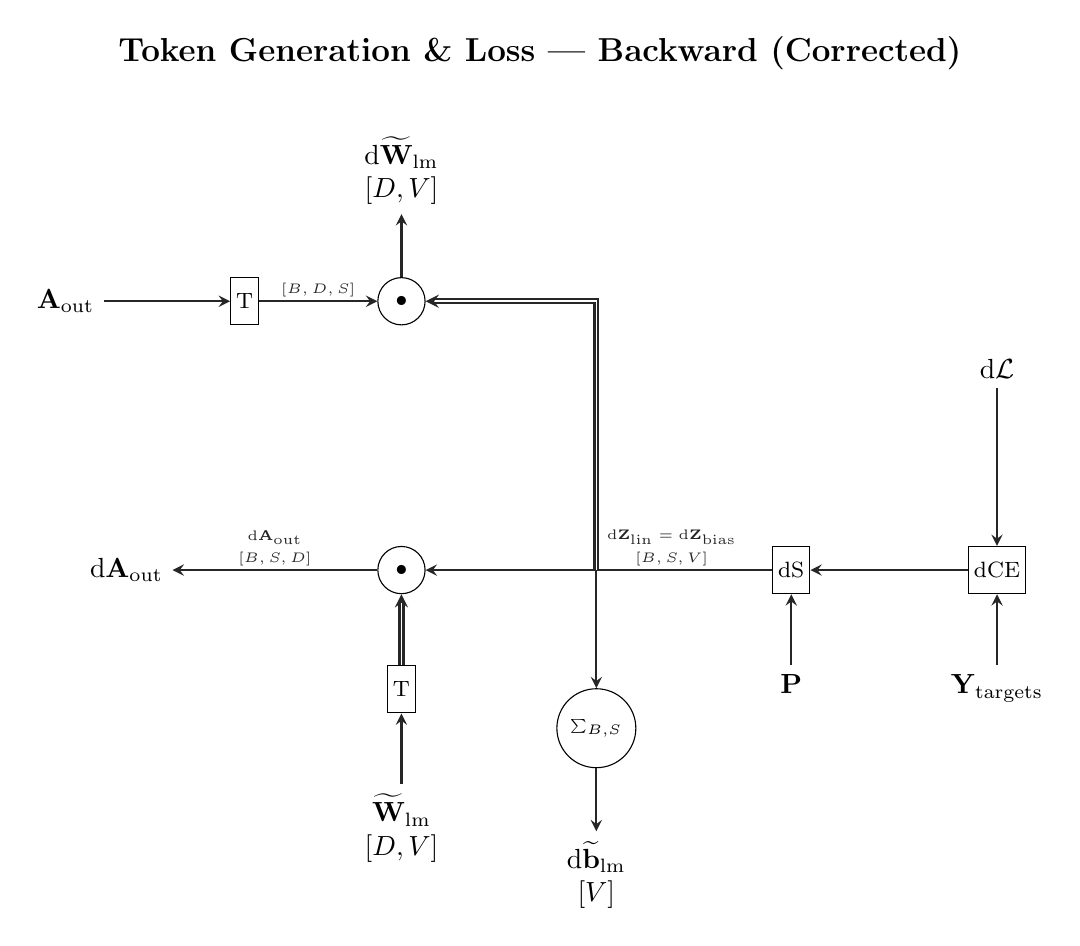
\begin{tikzpicture}[
  >=stealth,
  auxnode/.style={draw, rectangle, fill=white, minimum height=6mm, inner sep=2pt, font=\footnotesize, align=center},
  mulnode/.style={draw, circle, fill=white, minimum size=6mm, font=\footnotesize, align=center},
  addnode/.style={draw, circle, fill=white, minimum size=6mm, font=\footnotesize, align=center},
  sumnode/.style={draw, circle, fill=white, minimum size=6mm, font=\tiny, align=center},
  flow/.style={<-, thick, black!85},
  flow2/.style={double, <-, thick, black!85},
  fwd/.style={->, thick, black!85},
  gradflow/.style={->, thick, black!85},
  dimlabel/.style={font=\tiny, inner sep=1pt, align=center}
]

% Start from dL
\node           (dL)    at (18,0) {$\text{d}\mathcal{L}$};
\node[auxnode]  (dCE)   [below=2.0cm of dL] {dCE};
\node           (Y)     [below=0.9cm of dCE] {$\mathbf{Y_\text{targets}}$};

% Softmax backward
\node[auxnode]  (dS)   [left=2.0cm of dCE] {dS};
\node           (P)     [below=0.9cm of dS] {$\mathbf{P}$};

% Logits (Linear Projection) backprop node
\node[mulnode]  (backMul) [left=4.4cm of dS] {$\bullet$};
\node[auxnode]  (T_Wlm)   [below=0.9cm of backMul] {T};
\node           (Wlm)     [align=center, below=0.9cm of T_Wlm] {$\widetilde{\mathbf{W}}_{\text{lm}}$\\$[D,V]$};

\coordinate (B_split) at ($(backMul)!0.5!(dS)$);

% SUM node for Bias gradient
\node[sumnode]  (SumB) [below=1.5cm of B_split] {$\sum_{B,S}$};
\node           (db)   [align=center, below=0.8cm of SumB] {$\text{d}\widetilde{\mathbf{b}}_{\text{lm}}$\\$[V]$};

% dW calc
\node[mulnode]  (dWmul) [above=2.8cm of backMul] {$\bullet$};
\node[auxnode]  (TAout) [left=1.5cm of dWmul] {T};
\node           (Aout)  [left=1.6cm of TAout] {$\mathbf{A}_{\text{out}}$};
\node           (dW)    [align=center, above=0.8cm of dWmul] {$\text{d}\widetilde{\mathbf{W}}_{\text{lm}}$\\$[D,V]$};

% Back to Transformer
\node           (dH)    [left=2.6cm of backMul] {$\text{d}\mathbf{A}_{\text{out}}$};

% Flows
\draw[flow] (dCE) -- (dL);
\draw[fwd]  (Y) -- (dCE);
\draw[flow] (dS) -- (dCE);
\draw[fwd]  (P) -- (dS);

% Bias grad
\draw[gradflow] (B_split) -- (SumB.north);
\draw[gradflow] (SumB) -- (db);

% Linear projection backprop
\draw[flow] (backMul) -- (dS)
  node[dimlabel, pos=0.71, above]{\shortstack{$\text{d}\mathbf{Z}_{\text{lin}}=\text{d}\mathbf{Z}_{\text{bias}}$\\$[B,S,V]$}};
\draw[flow2] (backMul) -- (T_Wlm);
\draw[fwd]   (Wlm) -- (T_Wlm);
\draw[flow]  (dH) -- (backMul) node[dimlabel, midway, above]{\shortstack{$\text{d}\mathbf{A}_{\text{out}}$\\$[B,S,D]$}};

% dW calculation
\draw[gradflow] (dWmul) -- (dW);
\draw[fwd]  (Aout) -- (TAout);
\draw[fwd]  (TAout) -- (dWmul) node[dimlabel, midway, above]{\shortstack{$[B,D,S]$}};
\draw[flow2] (dWmul) -| (B_split);

\node[font=\large\bfseries, anchor=south]
  at ([yshift=6mm]current bounding box.north) {Token Generation \& Loss — Backward (Corrected)};
\end{tikzpicture}%
}

  \caption{출력 프로젝션과 손실의 역전파.
  손실로부터의 기울기는 소프트맥스와 교차 엔트로피를 거쳐
  로그릿으로 전달되고, 다시 언어 모델 프로젝션을 통해
  $\mathrm{d}\mathbf{A}_{\text{out}}$과
  파라미터 기울기 $\mathrm{d}\mathbf{W}_{\text{lm}}$,
  $\mathrm{d}\mathbf{b}_{\text{lm}}$를 만들어 낸다.}
  \label{fig:single_node_output_backward}
\end{figure}
